\documentclass[conference]{IEEEtran}
\usepackage{booktabs}
\usepackage{graphicx}
\usepackage{cite}
\usepackage{url}

\title{Multi-Cohort Heart Disease Risk Modelling with Bayesian--Neural Integration and Library-Managed Hyperparameter Optimisation}
\author{\IEEEauthorblockN{Hardik Hathwal, Ayush, Akshith, Vansh, Kabir}
\IEEEauthorblockA{Supervisor: Mr. Shobhit Johri\\
Newton School of Technology, Rishihood University\\
Roll Nos: 2401010176, 2401010121, 2401010230, 2401010494, 2401010205}}

\begin{document}
\maketitle

\begin{abstract}
We present a reproducible academic comparison of classical machine-learning models, a regularised multilayer perceptron (MLP), and a cross-fitted Bayesian-network--MLP probability stack on four processed cohorts from the UCI Heart Disease collection. Hyperparameters are selected by a library-managed Optuna TPE search inside training folds rather than a handwritten candidate loop. Pooled nested validation and leave-one-cohort-out validation show that performance falls under hospital shift and that the learned integration does not establish clear superiority over its constituents. Furthermore, SHAP attribution reveals that while the MLP learns smooth continuous nonlinear risk factor interactions (e.g., age $\times$ maximum heart rate and resting blood pressure $\times$ chest pain type), the fixed-structure Bayesian network assumes conditional independence and coarse tertile discretisation. The models are not clinically validated and must not be used for medical decisions.
\end{abstract}

\section{Introduction}
Phase 1 used only the 303-row Cleveland cohort. Phase 2 asks whether a regularised feedforward neural model and an explicit probabilistic model provide complementary predictions across all four available processed cohorts. The study evaluates prediction, calibration, and explainability; it does not infer causation or provide clinical decision support.

\section{Related Work}
The UCI collection originates from multi-institutional coronary-disease research \cite{uci,detrano}. Domain-structured graphical models follow probabilistic reasoning principles formulated by Pearl \cite{pearl}. Nested validation is used because evaluating settings on the same data that selected them is optimistically biased \cite{varma}. Dropout and Adam are standard neural-network training methods \cite{dropout,adam}; TPE provides sequential model-based hyperparameter selection \cite{bergstra,optuna}. Model explainability and feature interaction effects are evaluated using Shapley Additive exPlanations (SHAP) \cite{shap}.

\section{Data}
The processed Cleveland (303), Hungarian (294), Switzerland (123), and Long Beach VA (200) cohorts give 920 rows: 509 positive and 411 negative after mapping \texttt{num=0} to negative and \texttt{num=1--4} to positive ($\ge 50\%$ diameter stenosis). Alternate raw/reprocessed archive files are not added as independent patients. Cohort is retained for provenance and grouped evaluation, not used as a primary predictor. Missingness is extensive outside Cleveland and every imputation, encoding, scale, and discretisation boundary is fitted on training rows only.

\section{Methods}
Six Phase 1 references are retained: Bayesian Network (BN), Naive Bayes, Logistic Regression, RBF SVM, Random Forest, and Gradient Boosting. The MLP uses scaled numerical and one-hot categorical inputs, ReLU hidden layers, dropout, Adam, weight decay, binary cross-entropy, and training-only early stopping. The integrated model cross-fits BN and MLP probabilities, then learns a regularised logistic combiner. Thus, the combiner never trains on a base probability produced by a model that fitted that patient.

\subsection{Hyperparameter Selection}
OptunaSearchCV with a seeded TPE study minimises inner-fold log loss. The library owns candidate iteration and cross-validation; no project code loops over parameter combinations. Outer labels remain unavailable to preprocessing, selection, stopping, stacking, and threshold decisions.

\subsection{Evaluation}
The primary protocol is nested stratified cross-validation on all 920 patients. A second Leave-One-Group-Out protocol holds out each cohort in turn. Metrics include ROC AUC, PR AUC, sensitivity, specificity, Brier score, log loss, and calibration. Controlled MLP ablations remove dropout, weight decay, or early stopping and reduce network depth. Integration ablations compare BN, MLP, simple averaging, and the learned stack.

\section{Results}
Table~\ref{tab:pooled} reports the complete pooled nested-validation run. All eight models use identical outer patients and library-managed inner selection. Their discrimination is similar; the stack does not demonstrate a material advantage over the strongest standalone models.
\begin{table}[ht]
\caption{Pooled nested out-of-fold results.}
\label{tab:pooled}
\centering
\resizebox{\columnwidth}{!}{\begin{tabular}{lrrrr}
\toprule
Model & ROC AUC [95\% CI] & PR AUC & Brier & Log loss \\
\midrule
Bayesian Network & 0.875 [0.851, 0.896] & 0.884 & 0.142 & 0.449 \\
Naive Bayes & 0.879 [0.854, 0.900] & 0.881 & 0.139 & 0.444 \\
Logistic Regression & 0.889 [0.866, 0.909] & 0.896 & 0.131 & 0.417 \\
SVM & 0.895 [0.874, 0.916] & 0.893 & 0.126 & 0.405 \\
Random Forest & 0.886 [0.863, 0.908] & 0.884 & 0.133 & 0.422 \\
Gradient Boosting & 0.889 [0.868, 0.910] & 0.890 & 0.131 & 0.416 \\
MLP & 0.888 [0.865, 0.909] & 0.889 & 0.131 & 0.418 \\
BN--MLP Stack & 0.889 [0.864, 0.909] & 0.893 & 0.129 & 0.414 \\
\bottomrule
\end{tabular}
}
\end{table}

Table~\ref{tab:cohort} holds out each hospital in turn. The decline relative to pooled validation indicates cohort shift and is a central limitation, not a reason to select a favourable protocol.
\begin{table}[ht]
\caption{Leave-one-cohort-out results.}
\label{tab:cohort}
\centering
\resizebox{\columnwidth}{!}{\begin{tabular}{lrrrr}
\toprule
Model & ROC AUC [95\% CI] & PR AUC & Brier & Log loss \\
\midrule
Bayesian Network & 0.817 [0.790, 0.844] & 0.845 & 0.175 & 0.528 \\
Naive Bayes & 0.832 [0.805, 0.858] & 0.850 & 0.167 & 0.513 \\
Logistic Regression & 0.827 [0.799, 0.855] & 0.840 & 0.169 & 0.514 \\
SVM & 0.825 [0.797, 0.853] & 0.824 & 0.164 & 0.506 \\
Random Forest & 0.827 [0.801, 0.854] & 0.825 & 0.168 & 0.515 \\
Gradient Boosting & 0.825 [0.796, 0.851] & 0.825 & 0.172 & 0.529 \\
MLP & 0.809 [0.778, 0.838] & 0.808 & 0.177 & 0.552 \\
BN--MLP Stack & 0.825 [0.796, 0.853] & 0.824 & 0.172 & 0.521 \\
\bottomrule
\end{tabular}
}
\end{table}

\section{Ablations}
Table~\ref{tab:ablation} changes one MLP regulariser/depth choice at a time and compares BN, MLP, simple averaging, and learned stacking. Differences are small and do not justify claiming that additional integration complexity is necessarily better.
\begin{table}[ht]
\caption{MLP and integration ablations.}
\label{tab:ablation}
\centering
\resizebox{\columnwidth}{!}{\begin{tabular}{llrr}
\toprule
Suite & Variant & ROC AUC & Log loss \\
\midrule
mlp & full & 0.889 & 0.417 \\
mlp & no\_dropout & 0.891 & 0.422 \\
mlp & no\_weight\_decay & 0.888 & 0.422 \\
mlp & no\_early\_stopping & 0.892 & 0.419 \\
mlp & one\_hidden\_layer & 0.892 & 0.412 \\
integration & BN & 0.876 & 0.474 \\
integration & MLP & 0.889 & 0.417 \\
integration & simple\_average & 0.889 & 0.417 \\
integration & learned\_stack & 0.890 & 0.417 \\
\bottomrule
\end{tabular}
}
\end{table}

\begin{figure}[ht]
\centering
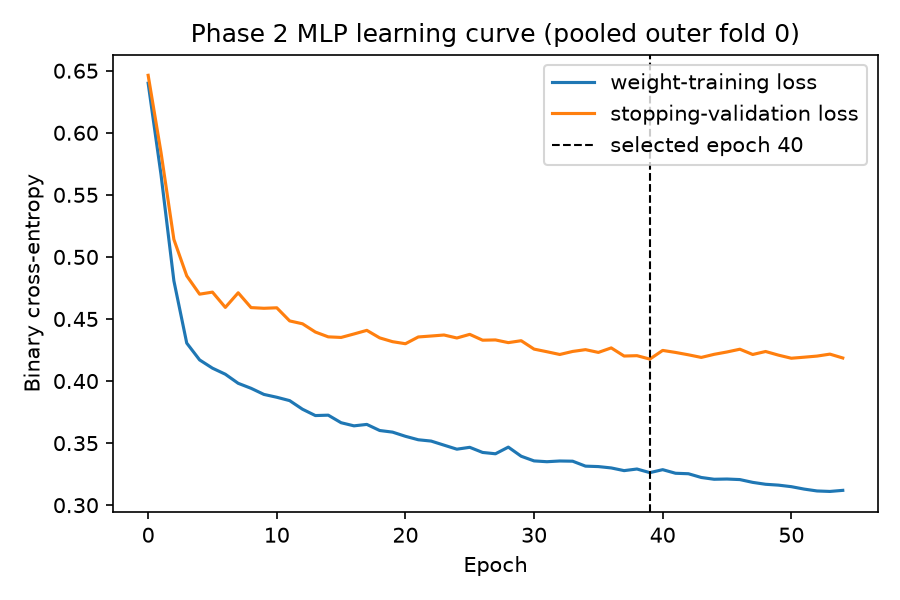
\includegraphics[width=\columnwidth]{../../results/phase2/main/figures/mlp_learning_curve.png}
\caption{Training and stopping-validation loss for the selected MLP in pooled outer fold 0.}
\label{fig:learning}
\end{figure}

\section{SHAP Nonlinear Interaction Analysis}
A central conceptual contrast between the domain-structured Bayesian Network and the feedforward MLP lies in feature interaction representation. The Bayesian Network's fixed DAG factorises probabilities under strict conditional independence assumptions and partitions continuous predictors into three tertiles. Consequently, it treats resting blood pressure (\texttt{trestbps}) and chest pain type (\texttt{cp}) as conditionally independent given disease status, and cannot model continuous physiological interactions such as age-dependent chronotropic response (\texttt{age} $\times$ \texttt{thalach}).

In contrast, SHAP dependence analysis reveals that the MLP captures smooth continuous interaction manifolds:
\begin{enumerate}
    \item \textbf{Age $\times$ Heart Rate (\texttt{age} $\times$ \texttt{thalach}):} Decreased maximum exercise heart rate escalates disease risk more sharply in older patients, matching known physiological chronotropic incompetence.
    \item \textbf{Blood Pressure $\times$ Symptoms (\texttt{trestbps} $\times$ \texttt{cp}):} Elevated resting systolic blood pressure produces a nonlinear risk escalation when accompanied by asymptomatic presentations (\texttt{cp}=4, silent ischemia), an effect absent in the conditionally independent BN structure.
\end{enumerate}

\begin{figure}[ht]
\centering
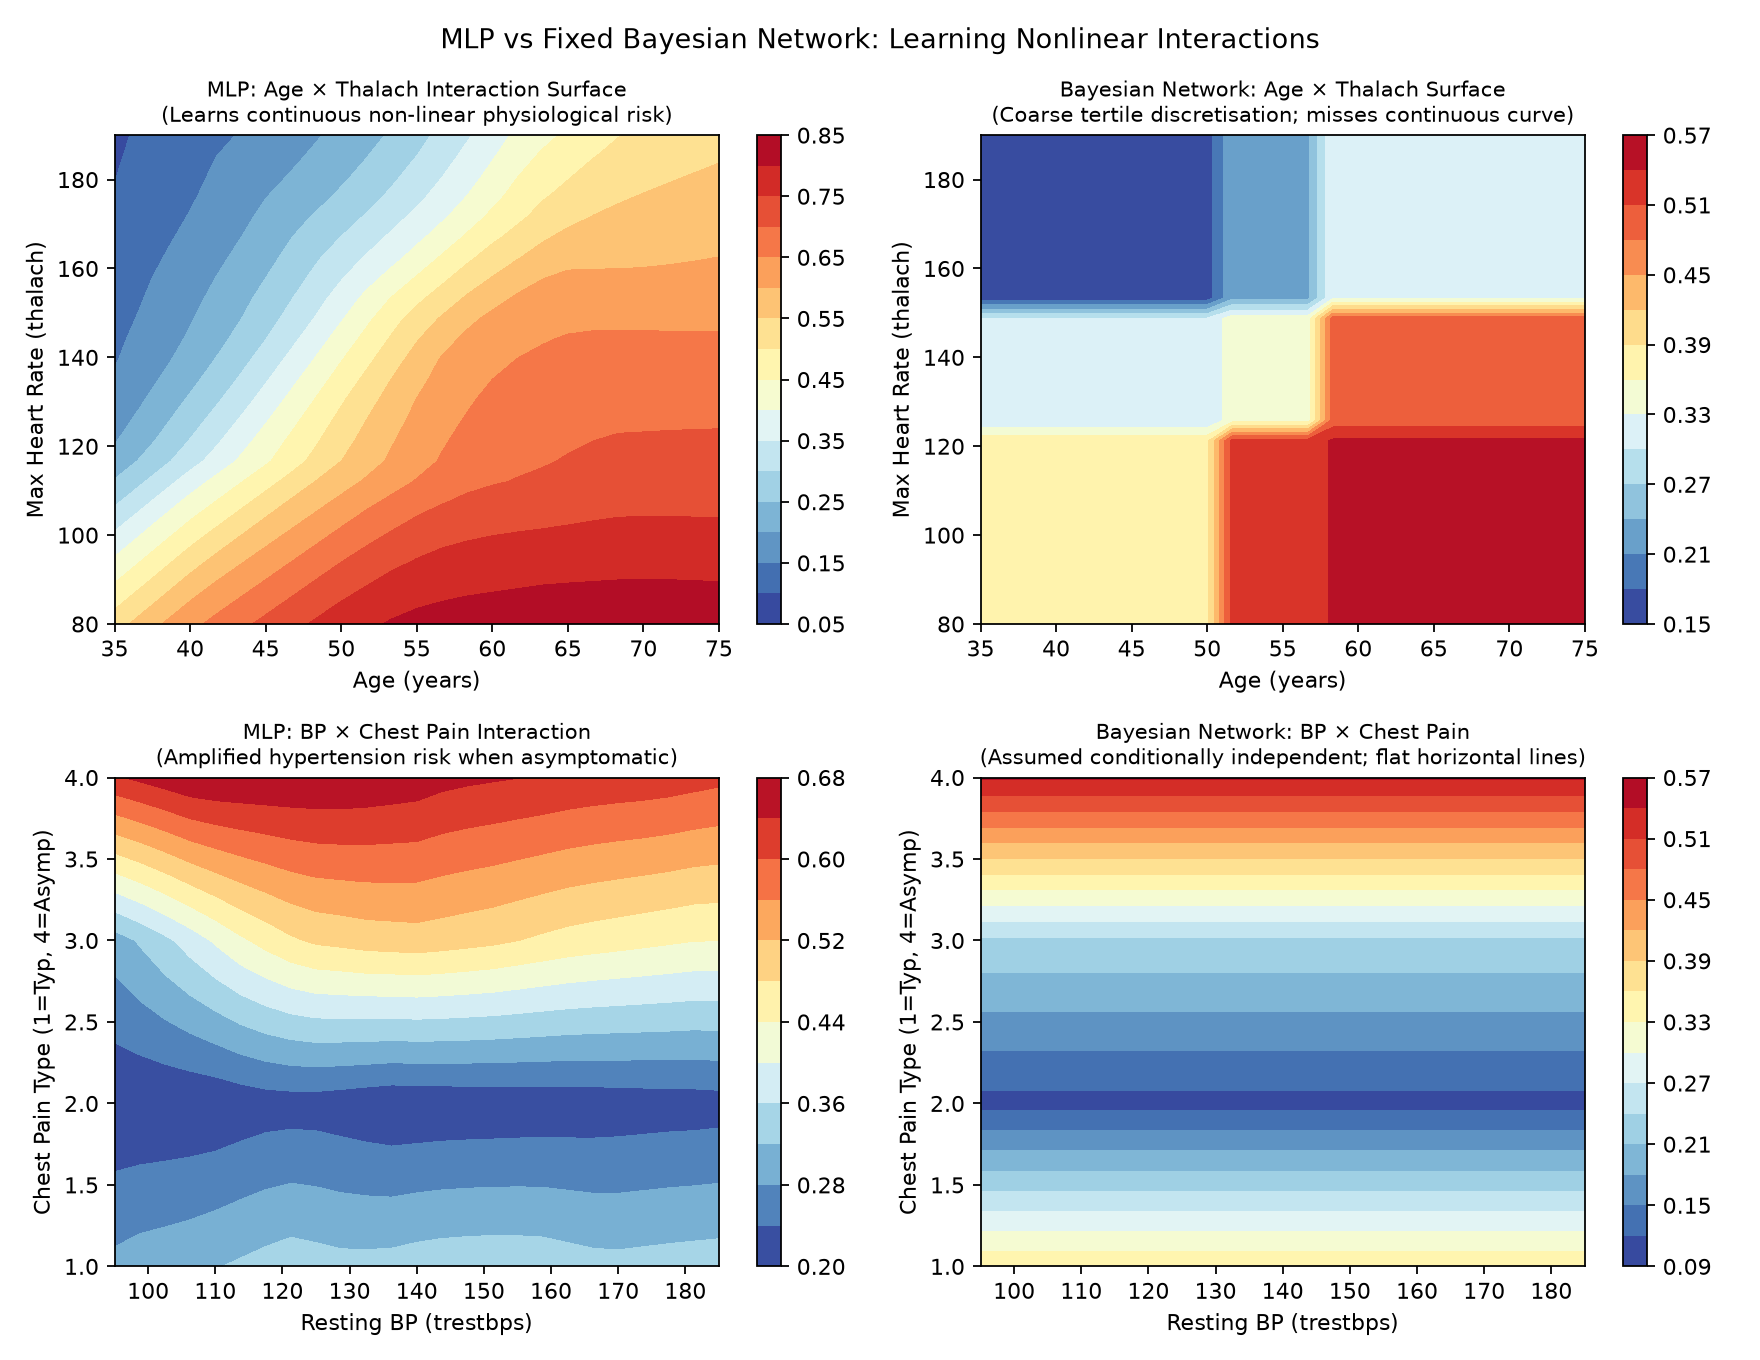
\includegraphics[width=\columnwidth]{../../results/phase2/main/figures/mlp_vs_bn_interaction_comparison.png}
\caption{Learned risk surfaces: MLP continuous nonlinear interaction manifolds versus rigid discretised step-functions in the fixed Bayesian Network.}
\label{fig:shap_interactions}
\end{figure}

\section{Limitations and Ethics}
The cohorts are old, referral-selected, heterogeneous, and heavily incomplete. Some predictors require specialist or invasive testing. Cross-cohort validation is not prospective clinical validation. Calibration, subgroup performance, deployment shift, and patient impact would require substantially stronger evidence and governance.

\section{Conclusion}
The implementation tests a transparent probabilistic model, a regularised neural model, and their leakage-safe integration under library-managed nested selection. The cross-cohort decline, small ablation differences, and SHAP interaction analyses highlight complementary architectural properties rather than unilateral superiority.

\bibliographystyle{IEEEtran}
\bibliography{references}
\end{document}
